\documentclass{article}

\usepackage{styles/arxiv}

\usepackage[utf8]{inputenc} % allow utf-8 input
\usepackage[T1]{fontenc}    % use 8-bit T1 fonts
\usepackage{hyperref}       % hyperlinks
\usepackage{url}            % simple URL typesetting
\usepackage{booktabs}       % professional-quality tables
\usepackage[english]{babel}
\usepackage{nicefrac}       % compact symbols for 1/2, etc.
\usepackage{microtype}      % microtypography
\usepackage{graphicx}
\usepackage{stmaryrd}

\usepackage{amsthm}
\usepackage{amssymb}
\usepackage{amsfonts}
\usepackage{amsmath}
\usepackage{mathtools}

\usepackage{tikz}
\usepackage{qtree}

\usepackage{listings}
\lstset{
  basicstyle=\itshape,
  xleftmargin=3em,
  literate={->}{$\rightarrow$}{2}
           {α}{$\alpha$}{1}
           {δ}{$\delta$}{1}
}

\usepackage{xstring}
\usepackage{stmaryrd}
\usepackage{wasysym}
\usepackage{textcomp}
\usepackage{blindtext}
\usepackage{subfiles}

\newtheorem{definition}{Definition}
\numberwithin{definition}{section}
\newtheorem{lemma}{Lemma}
\numberwithin{lemma}{section}
\newtheorem{proposition}{Proposition}
\numberwithin{proposition}{section}
\newtheorem{corollary}{Corollary}
\numberwithin{corollary}{section}
\newtheorem{theorem}{Theorem}
\numberwithin{theorem}{section}

\DeclareMathSymbol{\mathinvertedexclamationmark}{\mathclose}{operators}{'074}
\DeclareMathSymbol{\mathexclamationmark}{\mathclose}{operators}{'041}
\makeatletter
\newcommand{\raisedmathinvertedexclamationmark}{%
  \mathclose{\mathpalette\raised@mathinvertedexclamationmark\relax}%
}
\newcommand{\raised@mathinvertedexclamationmark}[2]{%
  \raisebox{\depth}{$\m@th#1\mathinvertedexclamationmark$}%
}
\begingroup\lccode`~=`! \lowercase{\endgroup
  \def~}{\@ifnextchar`{\raisedmathinvertedexclamationmark\@gobble}{\mathexclamationmark}}
\mathcode`!="8000
\makeatother

\newcommand{\intga}{\mathclap{\smash{\oplus}}{\int}}
\newcommand{\intgp}{\mathclap{\smash{\otimes}}{\int}}
\newcommand{\intgg}{\mathclap{\rightsquigarrow}\mathclap{\int}}

\title{Geometry of arithmetic expressions: I.\\ Basics and Problems}

%\date{Decmber 8, 2022}	% Here you can change the date presented in the paper title
%\date{} 				% Or removing it

\author{
  Mingli~Yuan \\
  AI Lab \\
  ColorfulClouds Tech.\\
  Beijing, 100083 \\
  \texttt{mingli.yuan@gmail.com}
}

% Uncomment to remove the date
%\date{}

% Uncomment to override  the `A preprint' in the header
\renewcommand{\headeright}{A preprint}
\renewcommand{\undertitle}{A preprint}

\begin{document}
\maketitle

\begin{abstract}
    TODO
\end{abstract}

\keywords{arithmetic expressions, hyperbolic geometry}

\setcounter{tocdepth}{2}
\tableofcontents
\newpage

\section{Introduction}\label{sec:introduction}

Can arithmetic expressions form a geometric space?
In this paper, the first in a series on the geometry of arithmetic expressions, we present several examples of arithmetic expression spaces and examine their properties.

Since this is a new area of research, we will begin by introducing a basic example in the first section.
Next, we will demonstrate more complex examples and discuss their properties and conclusions.

\subsection{Arithmetic expression}

In order to define arithmetic expressions involving real numbers in a rigorous way, we need to use a sophisticated type theory.
However, in order to keep things simple and maintain clarity, we will start by using only production rules,
but with certain semantic restrictions.

\begin{definition}
    The definition of arithmetic expression $a$ over $\mathbb{Q}$ is given by the following production rules:
    \begin{lstlisting}[mathescape]
    $a \longleftarrow x$
    $a \longleftarrow ( a + a )$
    $a \longleftarrow ( a - a )$
    $a \longleftarrow ( a \times a )$
    $a \longleftarrow ( a \div a )$
    \end{lstlisting}
    where $x \in \mathbb{Q}$, and we denote this as $a \in \mathbb{E} \left [\mathbb{Q} \right ]$.
\end{definition}

During the production process, we can obtain both a string representation and a tree representation of arithmetic expression $a$,
where the two representations are equivalent. For instance, the string representation of $a$ might be:

$$
(((((1 \times 2) \times 2) - 1) \times (2 + 1)) - 6)
$$

and the parsed syntax tree is depicted in Figure \ref{fig:syntaxtree}.

\begin{figure}[ht]
\centering
\resizebox{0.2\textheight}{!}{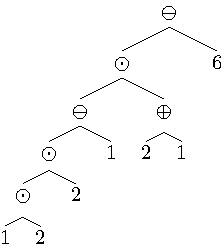
\includegraphics{images/02-example-expression-syntax-tree.pdf}}
\caption{a tree representation of an arithmetic expression}\label{fig:syntaxtree}
\end{figure}

We can easily obtain the string representation of $a$ from its tree representation by performing a pre-order traversal.
The concept of a \emph{sub-expression} can also be derived from the concept of a sub-tree.
The branch nodes are all labeled with operators: $+$, $-$, $\times$, $\div$. The leaf nodes are all labeled with numbers.

Evaluation $\nu$ is a partial function that operates on arithmetic expression $a \in \mathbb{E} \left [\mathbb{Q} \right ]$.
It is undefined only if division by zero occurs during the recursive evaluation process.

We can define evaluation $\nu(a)$ of $a$ recursively as follows:
\begin{itemize}
  \item Constant leaf: for any $x \in \mathbb{Q}$, $\nu(x) = x$.
  \item Compositional node by $+$: For any $(a + b)$, $\nu((a + b)) = \nu(a) + \nu(b)$.
  \item Compositional node by $-$: For any $(a - b)$, $\nu((a - b)) = \nu(a) - \nu(b)$.
  \item Compositional node by $\times$: For any $(a \times b)$, $\nu((a \times b)) = \nu(a) \nu(b)$.
  \item Compositional node by $\div$: For any $(a \div b)$, if $\nu(b) \neq 0$, then $\nu((a \div b)) = \nu(a) / \nu(b)$.
\end{itemize}

We say that an arithmetic expression $a$ is \emph{evaluable} if $\nu(a)$ is defined.
In the rest of this article, we will only consider evaluable arithmetic expressions unless stated otherwise.

Given an arithmetic expression $a$, we can obtain its tree representation.
If a node $l$ is a leaf node, its corresponding subexpression $s$ is a number, so we consider it to be already "evaluated".
If a node $b$ is a branch node, its corresponding subexpression $s$ is an expression, and we can apply $\nu$ to it to obtain a number $\nu(s)$.
During the recursive evaluation process, starting from the leaves and moving towards the root, the subexpressions are evaluated one after another.
However, the order of evaluations is generally not unique.

\begin{definition}
The evaluation order of an arithmetic expression $a$ is an ordering of branch nodes in the tree representation of $a$
such that every node (sub-expression) is evaluated before its parent.
\end{definition}

Below are examples of expressions that have a unique evaluation order. These include left-expanded, right-expanded,
and combinations of them, as shown in Figure \ref{fig:leftright} and Figure \ref{fig:combination}.

\begin{figure}[ht]
\centering
\resizebox{0.4\textheight}{!}{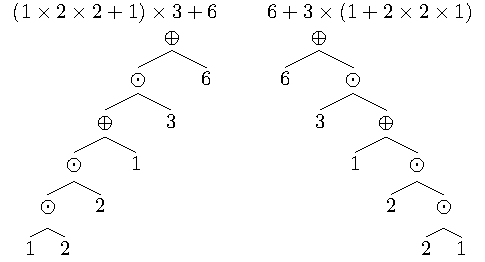
\includegraphics{images/03-example-expression-syntax-tree-left-right.pdf}}
\caption{right-expanded and left-expanded expressions}\label{fig:leftright}
\end{figure}

\begin{figure}[ht]
\centering
\resizebox{0.2\textheight}{!}{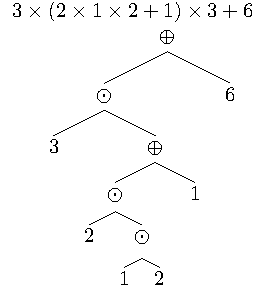
\includegraphics{images/04-example-expression-syntax-tree-combination}}
\caption{combinations of right-expanded and left-expanded expressions}\label{fig:combination}
\end{figure}

\begin{definition}
A threadlike expression is an arithmetic expression that all the right nodes in its tree representation are leaf nodes.
\end{definition}

So a threadlike expression is right-expanded and its evaluation order is unique.

Threadlike expressions are important because they are analogousness in the expression world to the concept of path in homotopy theory in geometry.

\subsection{An assignment and a grid}

Consider the upper half plane $\{\mathcal{H}: (x, y) | y > 0 \}$ equipped with an inner product and metrics defined as follows:

$$
\mathbf{a} \cdot \mathbf{b} = \begin{bmatrix} a_x & a_y \end{bmatrix} \begin{bmatrix} \frac{1}{y^2} & 0 \\ 0 & \frac{1}{y^2 \ln^2 2} \end{bmatrix} \begin{bmatrix} b_x \\ b_y \end{bmatrix}
$$

and

$$
ds^2 = \frac{1}{y^2} (dx^2 + \frac{dy^2}{\ln^2 2})
$$

We consider a scalar field satisfying

\begin{equation}
A = - \frac{x}{y}
\end{equation}

We call this field an \emph{assignment}.

Bridging by this scalar field, we can set up analogousness between path in homotopy and threadlike arithmetic expression
which is a special kind of arithmetic expression we will introduce in subsection \ref{sec:threadlike}.

\begin{figure}[ht]
\centering
\resizebox{0.9\textwidth}{!}{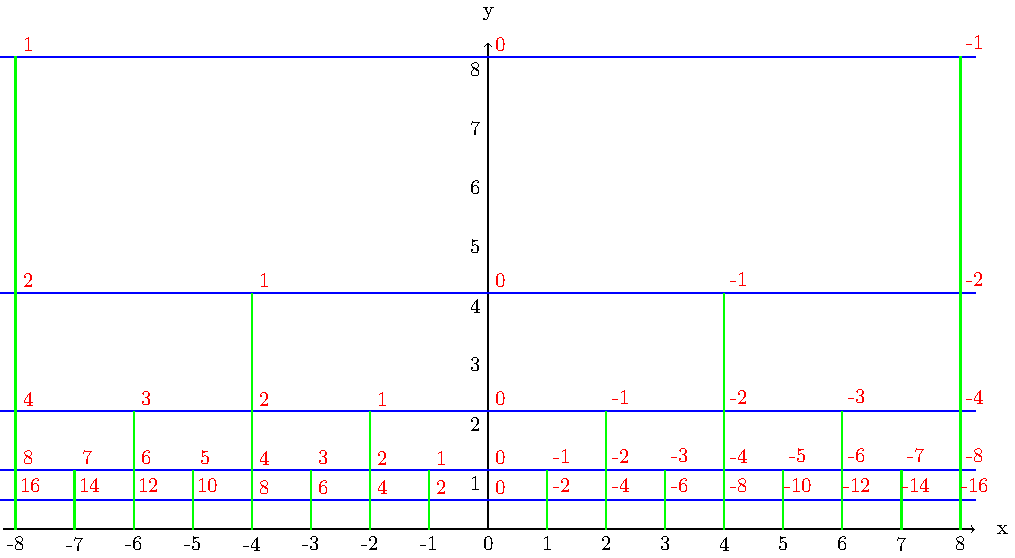
\includegraphics{images/01-grid-example-1.pdf}}
\caption{An addition-multiplication grid by generators with $\mu=1$ and $\lambda=\ln 2$}\label{fig:gridex0}
\end{figure}

We can draw a grid on the scalar field $A$ and underlying upper half plane $\mathcal{H}$ as shown in Figure \ref{fig:gridex0}.
The blue lines encode a $+ 1$ relationship, the green lines encode a $\times 2$ relationship,
and they are line families that are perpendicular to each other.
The length of the line segments between two neighboring crossing points are unit length(calculations in \ref{sec:unitlength}).
The red value at the crossing points is the value of the scalar field $A$ at that point.
Based on the relationships encoded by the lines, we can encode threadlike arithmetic expressions,
which will be introduced in the subsection \ref{sec:encoding}.

The addition-multiplication grid is also scale-invariant under the transformation
$$
\begin{cases}
x' = \alpha x\\
y' = \alpha y
\end{cases}
$$

where $\alpha = 2^k , k \in \mathbb{Z}$.

We can image if we make the grid finer and finer, the grid will become a continuous space.
This leads to a rigorous treatment of arithmetic expressions as a geometric space in subsection \ref{sec:topology}.

\subsection{Encoding threadlike expressions on the addition-multiplication gird}\label{sec:encoding}

If we interpret the horizontal blue lines as $+ 1$ and the vertical green lines as $\times 2$ in Figure \ref{fig:gridex0}, we can encode threadlike expressions on the addition-multiplication grid. For example, in Figure \ref{fig:encoding} we encode $(1 \times 4 - 1) \times 2 - 3$ as the bold black lines.

\begin{figure}[ht]
\centering
\resizebox{0.9\textwidth}{!}{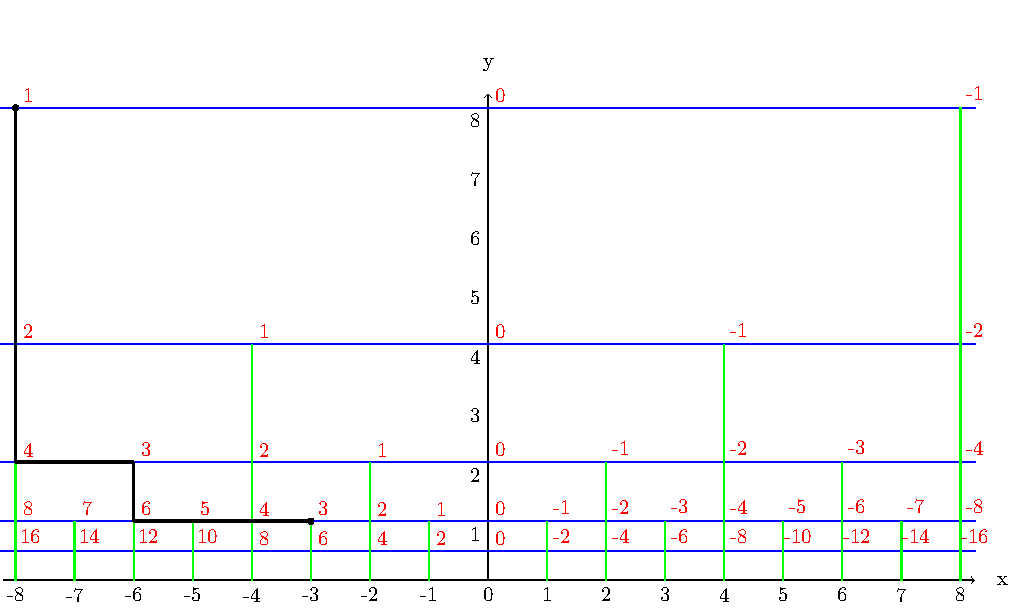
\includegraphics{images/05-example-expression-embedding}}
\caption{encoding threadlike expression}\label{fig:encoding}
\end{figure}

The zigzag lines in Figure \ref{fig:encoding} can be divided into four parts:
\begin{itemize}
\item the vertical line from $1$ to $4$: encoded as multiplication by $4$
\item the horizontal line from $4$ to $3$: encoded as subtraction by $1$
\item the vertical line from $3$ to $6$: encoded as multiplication by $2$
\item the horizontal line from $6$ to $3$: encoded as subtraction by $3$
\end{itemize}

\subsection{From a scalar field to a space of threadlike expressions}

As shown in Figure \ref{fig:canonicalform}, we have the following paths and expressions:
\begin{itemize}
\item the black path: $1 \times 8 - 5 = 3$
\item the purple path: $(1 - \frac{5}{8}) \times 8 = 3$
\item the brown path: $(((1 - \frac{1}{8}) \times 2 - \frac{1}{2}) \times 2 - 1) \times 2 = 3$
\item the orange path: infinit many addition-multiplication terms accumulated together, a special kind of integration
\end{itemize}

\begin{figure}[ht]
\centering
\resizebox{0.9\textwidth}{!}{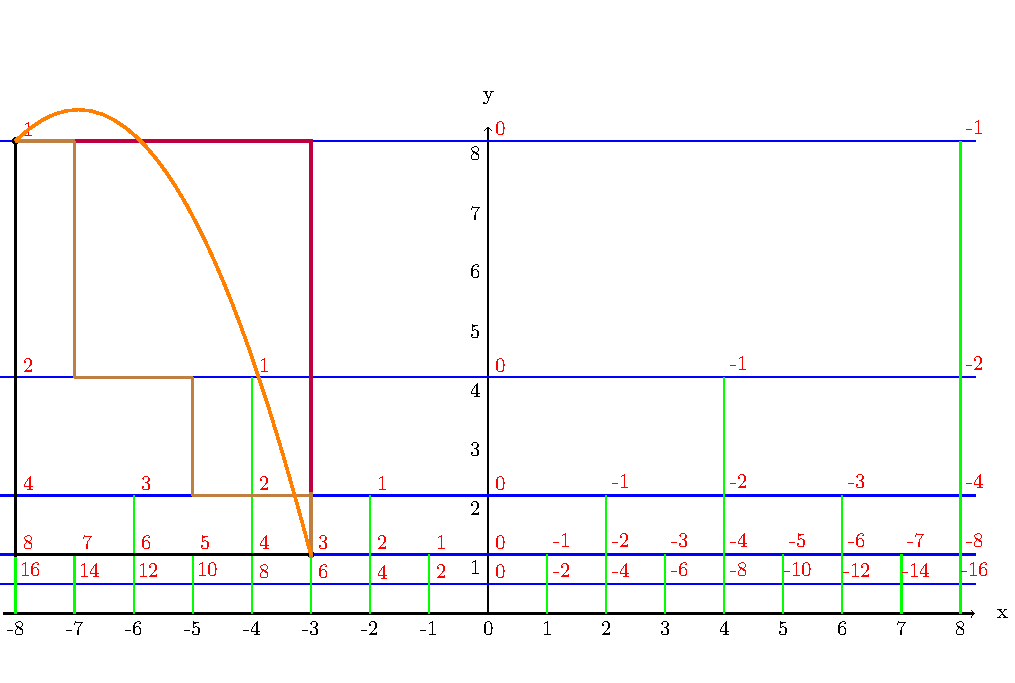
\includegraphics{images/06-example-canonical-form}}
\caption{different encodings and their canonical form}\label{fig:canonicalform}
\end{figure}

All of the paths in Figure \ref{fig:canonicalform} have the same source $1$ and same target $3$. We will discuss a canonical form for these paths.

It is easy to see that the expressions can be transformed into each other by using the multiplication distributive law and by combining and decomposing terms.

Conversion form brown path to black path
\begin{align}
3 & = (((1 - \frac{1}{8}) \times 2 - \frac{1}{2}) \times 2 - 1) \times 2 \\
& = 1 \times 8 -  \frac{1}{8} \times 8 - \frac{1}{2} \times 4 - 1 \times 2 \\
& = 1 \times 8 - 5
\end{align}

Conversion form brown path to purple path
\begin{align}
3 & = (((1 - \frac{1}{8}) \times 2 - \frac{1}{2}) \times 2 - 1) \times 2 \\
& = (1 - \frac{1}{8}) \times 8 - \frac{1}{2} \times 4 -  1 \times 2 \\
& = (1 - \frac{1}{8}) \times 8 - \frac{1}{4} \times 8 -  \frac{1}{4} \times 8 \\
& = (1 - \frac{1}{8} - \frac{1}{4} - \frac{1}{4}) \times 8 \\
& = (1 - \frac{5}{8}) \times 8
\end{align}

Therefore, we can define the black and purple paths in Figure \ref{fig:canonicalform} as a pair of canonical paths,
which represent all threadlike expressions connecting the source $1$ and the target $3$.

Once we have such canonical paths, we can determine the canonical form of the whole space relative to an arbitrary source point $O$
and any other target point $P$. This allows us to define the space as a space of threadlike expressions.

\subsection{Topological arithmetica expression space}\label{sec:topology}

\newpage

\section{Flow equation and its conclusion}\label{sec:flowequation}

\subsection{Flow equation}\label{sec:equation}

Consider an infinitesimal generation process over a Riemannian surface $M$ with one generator for an additional action $\mu$ and the other for a multiplicative action $e^\lambda$. These two generators are perpendicular. Under this generation process, we obtain an assignment $A: M \to R$ over the surface.

At any point with an assignment $a_0$, considering a movement with a distance of $\epsilon$, direction angle of $\theta$, and time elapsed of $\delta$, we can establish the following:

\begin{equation}
    a_{\delta} = (a_0 + \mu \epsilon \cos \theta)e^{\lambda \epsilon \sin \theta}
\end{equation}

or

\begin{equation}
    a_{\delta} = a_0 e^{\lambda \epsilon \sin \theta} + \mu \epsilon \cos \theta
\end{equation}

Both can be simplified to the same

\begin{equation}
    a_{\delta} = a_0 + \epsilon (a_0 \lambda \sin \theta + \mu \cos \theta)
\end{equation}

Then

\begin{equation}
    \frac{1}{\delta} (a_{\delta} - a_0) = \frac{\epsilon}{\delta} (\mu \cos \theta + x_0 \lambda \sin \theta)
\end{equation}

When both $\delta$ and $\epsilon$ are towards zero, we get $da / dt$, and hence

\begin{equation}
    \frac{da}{dt} = u (\mu \cos \theta + a \lambda \sin \theta)
\end{equation}

Or, we can change it to other forms

\begin{equation}
    \frac{da}{ds} = \mu \cos \theta + a \lambda \sin \theta\label{eq:flow}
\end{equation}

The left side of the flow equation (\eqref{eq:flow}) is governed by the distance structure, and the right side is governed by the angle structure. This leads to a theorem.

\begin{theorem}
Isometries keep the flow equation\eqref{eq:flow}
\label{thm:isometry}
\end{theorem}

\subsection{The contour-gradient form of flow equation}

It is easy to derive the contour equation in the local coordinate

\begin{equation}
    \mu \cos \theta_c + a \lambda \sin \theta_c = 0
\end{equation}

then we have

\begin{equation}
    \theta_c = - \arctan \frac{\mu}{a \lambda}
\end{equation}

the contour and the gradient are perpendicular to each other

\begin{equation}
    \theta_g = \pm \frac{\pi}{2} - \arctan \frac{\mu}{a \lambda}
\end{equation}

then along $\theta_g$ we have

\begin{equation}
    \frac{da}{ds} = \mu \cos (\pm \frac{\pi}{2} - \arctan \frac{\mu}{a \lambda}) + a \lambda \sin (\pm \frac{\pi}{2} - \arctan \frac{\mu}{a \lambda})
\end{equation}

\begin{equation}
    \frac{da}{ds} = \pm \sqrt{\mu^2 + \lambda^2 a^2}\label{eq:grad}
\end{equation}

Equation \eqref{eq:grad} is solvable, and we get the relation between $a$ and $s$ along the gradient flow line:

\begin{equation}
    \pm \tanh(\lambda s + c) = \frac{\lambda a}{\sqrt{\mu^2 + \lambda^2 a^2}}
\end{equation}

If we assume $\mu > 0$, we can further simplify the equation

\begin{equation}
  a = \pm \frac{\mu}{\lambda} \sinh(c \pm \lambda s)\label{eq:gradevo}
\end{equation}

By introducing the right-hand rotation angle $\phi$ along the gradient direction, we can establish a local polar coordinate system based on the gradient and contour lines.
Then the growth rate of $a$ along the angle $\phi$ is

\begin{equation}
    \frac{da}{ds} = \mu \cos (\frac{\pi}{2} - \arctan \frac{\mu}{a \lambda} + \phi) + a \lambda \sin (\frac{\pi}{2} - \arctan \frac{\mu}{a \lambda} + \phi)
    \label{eq:fourfold}
\end{equation}

And the simplified equation is

\begin{equation}
    \frac{da}{ds} = \sqrt {\mu^2 + a^2 \lambda^2} \cos \phi\label{eq:contourgradient}
\end{equation}

The equation \eqref{eq:contourgradient} is the flow equation in the contour-gradient coordinate system.

In this coordinate system, the addition line and the multiplication line are:

\begin{equation}
    \phi = \arccos \frac{\mu}{\sqrt {\mu^2 + a^2 \lambda^2}} \label{eq:additionalline}
\end{equation}

\begin{equation}
    \phi = \arccos \frac{a \lambda}{\sqrt {\mu^2 + a^2 \lambda^2}}\label {eq:mulitiplcativeline}
\end{equation}

By analyzing the formula, we can also get the geometric meaning of the assignment.
On the hyperbolic plane with sectional curvature $\kappa$, the area of the circle with radius $r$ is given by the following formula

\begin{equation}
2 \pi \int_0^r \left(\frac{\sinh(\sqrt{\kappa} t)}{\sqrt{\kappa}}\right) \, \mathrm{d}t\label{eq:circlearea}
\end{equation}

Notice that the similarity between equation \ref{eq:gradevo} and equation \ref{eq:circlearea} when $c=0$ will lead us to
the next subsection of the geometric interpretation of the formula.

\subsection{Geometric interpretation of the formula}

\newpage

\section{The first kind of arithmetic expression space}\label{sec:firstkind}

\subsection{Example I}\label{subsec:exmp1}

\begin{theorem}\footnote{The proof is originally by Le Zhang, and modified by Mingli Yuan}
For the above $A$, $A$ satisfy the flow equation\eqref{eq:flow}
\end{theorem}

\begin{proof}
$$
da = d(-\frac{x}{y}) = \frac{xdy - ydx}{y^2} = -\frac{dx + ady}{y}
$$

and

$$
ds = \frac{\sqrt{dx^2 + dy^2}}{y}
$$

then

$$
\frac{da}{ds} = - \frac{dx + ady}{y} \frac{y}{\sqrt{dx^2 + dy^2}} = - \frac{dx + ady}{\sqrt{dx^2 + dy^2}}
$$

Considering the local coordinate is given by $(-1, 0)$ and $(0, -1)$ under the right-hand rule, we have

$$
\cos \theta = \frac{\begin{bmatrix} dx & dy \end{bmatrix} \begin{bmatrix} \frac{1}{y^2} & 0 \\ 0 & \frac{1}{y^2} \end{bmatrix} \begin{bmatrix} -1 \\ 0 \end{bmatrix}}{\sqrt{\begin{bmatrix} dx & dy \end{bmatrix} \begin{bmatrix} \frac{1}{y^2} & 0 \\ 0 & \frac{1}{y^2} \end{bmatrix} \begin{bmatrix} dx \\ dy \end{bmatrix}}\sqrt{\begin{bmatrix} -1 & 0 \end{bmatrix} \begin{bmatrix} \frac{1}{y^2} & 0 \\ 0 & \frac{1}{y^2} \end{bmatrix} \begin{bmatrix} -1 \\ 0 \end{bmatrix}}}
$$

hence

$$
\cos \theta = \frac{-dx}{\sqrt{dx^2 + dy^2}}
$$

and similarly

$$
\sin \theta = \frac{-dy}{\sqrt{dx^2 + dy^2}}
$$

then

$$
\frac{da}{ds} = \cos \theta + a \sin \theta
$$

\end{proof}

\subsubsection{As eigenvalue of Laplacian}

We can verify $A$ is an eigenvalue of the Laplacian

$$
\Delta A = - y^2 (\frac{\partial^2}{\partial x^2} A + \frac{\partial^2}{\partial y^2} A) = y^2 (\frac{1}{\partial y} (\frac{1}{\partial y} \frac{x}{y})) = 2 A
$$

\subsection{Example II}\label{subsec:exmp2}

\subsubsection{Geometry settings}\label{subsec:gsetting2}

First, we introduce the horocycle-based coordinate system of hyperbolic surfaces.
It is a global coordinate system given by two orthogonal pencils of circles; one pencil are horocycles sharing the same ideal point,
the other are geodesics which are perpendicular to the first pencil.

On the Poincaré disc $\mathcal{P}$, the blue horocycles are tangible each other at the ideal point $\Omega$, which forms the first pencil,
the green lines are geodesics forms the second pencil; and the coordinate of point $P$ are given by the length of $OQ$ and $QP$,
where the point $O$ is the origin and the length is the metric inside the hyperbolic surface.

The coordinate of $P$ is $(u,v)$ where the sign of the length is decided by below rules:
\begin{itemize}
    \item u: if $P$ is in the same side of $\Omega$, then x is positive; otherwise x is negative
    \item v: the sign of the length should satisfy the right-hand rule
\end{itemize}

\begin{figure}[ht]
\centering
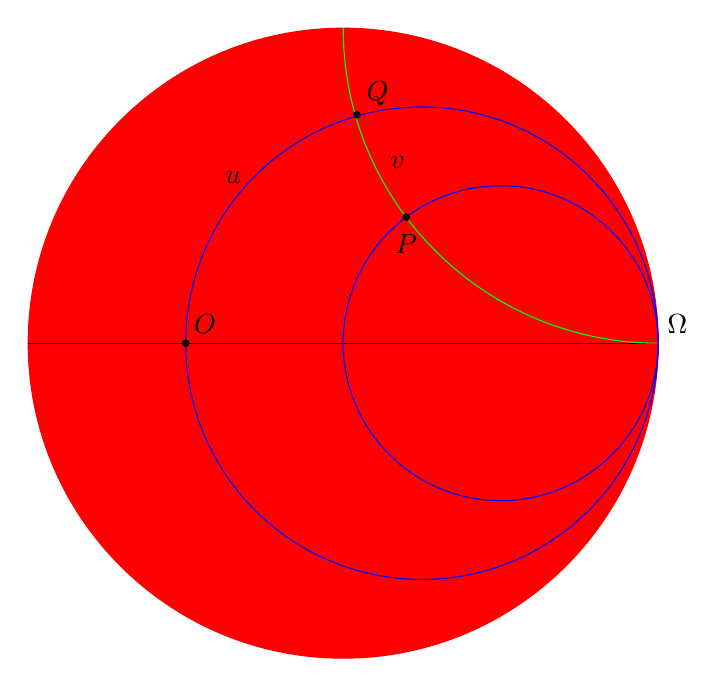
\begin{tikzpicture}
    \node[anchor=225] at (4,2) {$\Omega$};
    \draw[red,fill=red] (0,2) circle[radius=4];
    \draw[blue] (1, 2) circle[radius=3];
    \draw[black] (-4,2) -- (4,2);
    \draw[green] (4,2) arc (-90:-180:4);
    \draw[blue] (2, 2) circle[radius=2];
    \node[fill,circle,inner sep=1pt] at (-2,2) {};
    \node[anchor=225] at (-2,2) {$O$};
    \node[fill,circle,inner sep=1pt] at (0.175,4.9) {};
    \node[anchor=225] at (0.175,4.9) {$Q$};
    \node[fill,circle,inner sep=1pt] at (0.8,3.6) {};
    \node[anchor=90] at (0.8,3.5) {$P$};
    \node[anchor=225] at (0.49,4.1) {$v$};
    \node[anchor=225] at (-1.6,3.9) {$u$};
\end{tikzpicture}
\caption{Horocycle-based coordinate system}\label{fig:horocyclecoord}
\end{figure}

We can equip it with an inner product

\[
\mathbf{a} \cdot \mathbf{b} = \begin{bmatrix} a_u & a_v \end{bmatrix} \begin{bmatrix} e^{-2v} & 0 \\ 0 & 1 \end{bmatrix} \begin{bmatrix} b_u \\ b_v \end{bmatrix}
\]

and the metrics

$$
ds^2 = e^{-2v} du^2 + dv^2
$$

\subsubsection{The assignment}

\begin{equation}
A = u e^{-v}
\end{equation}

\begin{theorem}
For the above $A$, $A$ satisfy the flow equation\eqref{eq:flow}
\end{theorem}

\begin{figure}[ht]
\centering
\begin{tikzpicture}
\draw [black, line width=0.6pt, ->] (0,0) to[out=90,in=270] (0,4.25);
\node [anchor=south] at (0,4.5) {y};
\draw [black, line width=0.6pt, ->] (-4.25,0) to[out=0,in=180] (4.25,0);
\node [anchor=west] at (4.5,0) {x};

\draw [blue, line width=0.6pt] (-4.25,4.0) to[out=0,in=180] (4.25,4.0);
\draw [blue, line width=0.6pt] (-4.25,2.0) to[out=0,in=180] (4.25,2.0);
\draw [green, line width=0.6pt] (-3.5,0) to[out=90,in=270] (-3.5,4.5);

\node[anchor=45] at (0.0,4.0) {$O$};
\node[anchor=45] at (-3.5,4.0) {$Q$};
\node[anchor=45] at (-3.5,2.0) {$P$};
\node[anchor=225] at (-2.0,4.1) {$x = u$};
\node[anchor=225] at (-3.0,1.0) {$y = e^v$};

\end{tikzpicture}

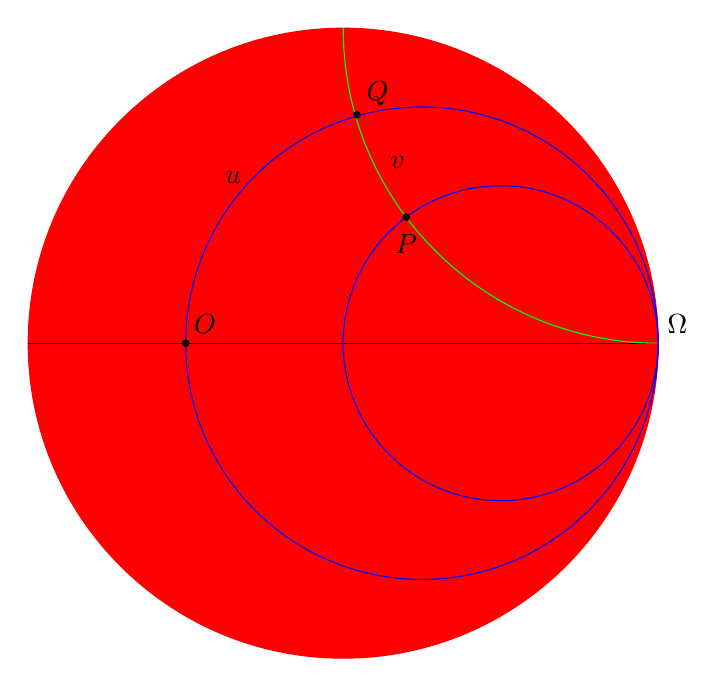
\begin{tikzpicture}
    \node[anchor=225] at (4,2) {$\Omega$};
    \draw[red,fill=red] (0,2) circle[radius=4];
    \draw[blue] (1, 2) circle[radius=3];
    \draw[black] (-4,2) -- (4,2);
    \draw[green] (4,2) arc (-90:-180:4);
    \draw[blue] (2, 2) circle[radius=2];
    \node[fill,circle,inner sep=1pt] at (-2,2) {};
    \node[anchor=225] at (-2,2) {$O$};
    \node[fill,circle,inner sep=1pt] at (0.175,4.9) {};
    \node[anchor=225] at (0.175,4.9) {$Q$};
    \node[fill,circle,inner sep=1pt] at (0.8,3.6) {};
    \node[anchor=90] at (0.8,3.5) {$P$};
    \node[anchor=225] at (0.49,4.1) {$v$};
    \node[anchor=225] at (-1.6,3.9) {$u$};
\end{tikzpicture}
\caption{Mapping between two examples}\label{fig:mapping}
\end{figure}

\begin{proof}

For example in last section \ref{subsec:exmp1}, if we introduce complex

$$
z = x + y i
$$

and there is a Möbius transform

$$
z \mapsto \frac{z-i}{z+i}
$$

that can connect the upper half plane model in last section \ref{subsec:exmp1} to current Horocycle-based coordinate system.

This transform maps each horizontal lines in $\mathcal{H}$ into the horocycles sharing the same ideal point $\Omega = 1$ in $\mathcal{P}$,
also it maps each vertical geodesics in $\mathcal{H}$ into geodesics in $\mathcal{P}$ which are perpendicular to the above horocycles.

And rewrite the Möbius transform in the target coordinate, we get:

$$
\begin{cases}
x = u\\
y = e^v \\
\end{cases}
$$

This lead to

$$
A = -\frac{x}{y} = u e^{-v}
$$

And because of theorem \ref{thm:isometry} and Möbius transform is conformal, we can conclude that $A = u e^{-v}$ obey flow equation.

\end{proof}

\subsubsection{As eigenvalue of Laplacian}

Laplacian is given by\cite{Costa2001ADO}

$$
\Delta = e^{2y} \frac{\partial^2}{{\partial x}^2} + \frac{\partial^2}{{\partial y}^2} - \frac{\partial}{\partial y}
$$

and we have $A$ is an eigenvalue of the Laplacian
$$
\Delta A = e^{2y} \frac{\partial^2(x e^{-y})}{{\partial x}^2} + \frac{\partial^2(x e^{-y})}{{\partial y}^2} - \frac{\partial(x e^{-y})}{\partial y} = 2A
$$

\subsection{Equivalence of the two examples}

\subsection{Generators independence}

\newpage

\section{Threadlike arithmetic expressions with two generator}\label{sec:expressions}
For a number field $\mathcal{F}$ and $\mu, \lambda \in \mathcal{F}$, we consider the arithmetical expression set
$E(\mu, \lambda)$ which is freely generated from
\begin{itemize}
    \item initial operand: $0$
    \item operator: $\odot: x \mapsto x$
    \item operator: $\oplus_\mu: x \mapsto x + \mu$
    \item operator: $\ominus_\mu: x \mapsto x - \mu$
    \item operator: $\otimes_\lambda: x \mapsto x \cdot e^\lambda$
    \item operator: $\oslash_\lambda: x \mapsto x / e^\lambda$
\end{itemize}

$\mu$ is the additional generator and $\lambda$ is the multiplicative generator.
We may omit $\mu$ and $\lambda$ from the index notation when context is clear.

With different equality we adopt on $E(\mu, \lambda)$, we will get different structures:
\begin{itemize}
    \item literal structure: under the literal equality which leads to paths on a generative tree structure
    \item syntactical structure: under the syntactical equality which embrace a path group
    \item semantical structure: under the equality of numbers after evaluating both sides of equality comparison into values
\end{itemize}

\subsection{Literal structure}\label{subsec:literial}

When we adopt literal equality, we get a generative tree structure with degree 5.

\begin{itemize}
    \item root: initial operand $0$
    \item edge: each node have $5$ edge with symbols $\odot$, $\oplus$, $\ominus$, $\otimes$ and $\oslash$ as children
\end{itemize}

The path from root to any node is an arithmetical expression. A different path is a different expression in literal equality.

\begin{figure}[ht]
\centering
\Tree
[.0
    [.$\odot$   [.$\odot$ ] [.$\oplus$ ] [.$\ominus$ ] [.$\otimes$ ] [.$\oslash$ ] ]
    [.$\oplus$  [.$\odot$ ] [.$\oplus$ ] [.$\ominus$ ] [.$\otimes$ ] [.$\oslash$ ] ]
    [.$\ominus$ [.$\odot$ ] [.$\oplus$ ] [.$\ominus$ ] [.$\otimes$ ] [.$\oslash$ ] ]
    [.$\otimes$ [.$\odot$ ] [.$\oplus$ ] [.$\ominus$ ] [.$\otimes$ ] [.$\oslash$ ] ]
    [.$\oslash$ [.$\odot$ ] [.$\oplus$ ] [.$\ominus$ ] [.$\otimes$ ] [.$\oslash$ ] ]
]
\caption{Generative tree of literal structure}
\end{figure}

Suppose we have a series of operators $a_1, a_2, \cdots a_{n-1}, a_n$, we introduce a \emph{path notion}.

\begin{definition}
\label{definition:path}
    a path of operators $a_1 a_2 \cdots a_{n-1} a_n$ is a function over $\mathcal{F}$ which apply operators on an operand in turn
    $$a_1 a_2 \cdots a_{n-1} a_n (x) \coloneqq a_n( a_{n-1}( \cdots a_2( a_1(x) ) \cdots ) ), \forall x \in \mathcal{F}$$
\end{definition}

Any expressions in $E(\mu, \lambda)$ can be written as a path with operand $0$. And now we verify the operators is associative inside a path.

\begin{lemma}
\label{lemma:associative}
    The operators inside a path is associative, i.e. $$x (y z) = (x y) z$$
\end{lemma}

\begin{proof}
    Follow the definition, we have
$$(x (y z)) [\alpha] = (y z) (x[\alpha]) = z(y(x[\alpha]))$$
$$((x y) z) [\alpha] = z ((x y)[\alpha]) = z(y(x[\alpha]))$$
\qedhere
\end{proof}

\begin{definition}
\label{definition:concatenate}
    Concatenate of paths $p_1 \cdot p_2$ is defined as the composite of functions
    $$p_1 \cdot p_2 \coloneqq p_2 \circ p_1 $$
\end{definition}

\begin{theorem}
\label{theorem:semigroup}
the algebraic structure $\mathcal{P} = (E, \cdot)$ is a semigroup.
\end{theorem}

\subsection{Syntactical structure}\label{subsec:syntactical}

We can introduce the inverse notion
\begin{itemize}
    \item $\oplus^{-1} = \ominus$
    \item $\ominus^{-1} = \oplus$
    \item $\otimes^{-1} = \oslash$
    \item $\oslash^{-1} = \otimes$
    \item $\odot^{-1} = \odot$
\end{itemize}

Then we have the calculation rule of inverse.

\begin{lemma}
\label{lemma:inverserule}
If we have
$$\beta = \alpha a_1 a_2 \cdots a_{n-1} a_n$$
then
$$\alpha = \beta a_n^{-1} a_{n-1}^{-1} \cdots a_2^{-1} a_1^{-1}$$
\end{lemma}

\begin{proof}
Notice that $\oplus, \ominus, \otimes, \oslash$ are all bijections, we know that $\alpha a_1 a_2 \cdots a_{n-1} a_n$ is a composition of functions

$$\beta = a_n( a_{n-1}( \cdots a_2( a_1(\alpha) ) \cdots ) )$$

Considering the inverse of a composition, we have

$$\alpha = a_1^{-1}( a_2^{-1}( \cdots a_{n-1}^{-1}( a_n^{-1}(\beta) ) \cdots ) )$$

Or under the path notion

$$\alpha = \beta a_n^{-1} a_{n-1}^{-1} \cdots a_2^{-1} a_1^{-1}$$

\qedhere
\end{proof}

Informally we can divide a long calculation into pieces, or composite small pieces of calculations into a longer one,
for example

$$\gamma = 0 a_1 a_2 \cdots a_{n-1} a b_1 b2 \cdots b_{m-1} b_m$$

can be rewritten as

$$\gamma = 0 ((\odot a_1 a_2 \cdots a_{n-1} a) \circ (\odot b_1 b_2 \cdots b_{m-1} b_m))$$

And if we treat $\odot$ and $0$ as the same, and we define

$$\alpha = 0 a_1 a_2 \cdots a_{n-1} a$$
$$\beta = 0 b_1 b2 \cdots b_{m-1} b_m$$

We have

$$\gamma = \alpha \circ \beta$$

where $\alpha$, $\beta$ and $\gamma$ are all well defined in $E$.

Under such definition, the algebraic structure $\mathcal{P} = (E, \circ)$ is a group, and we call it \emph{path group}.

\begin{theorem}
\label{theorem:pathgroup}
the algebraic structure $\mathcal{P} = (E, \circ)$ is a group
\end{theorem}

\begin{proof}
    Follow the definition of group, we have
\qedhere
\end{proof}

The cayley tree of path group $\mathcal{P}$ is a tree structure as below

\begin{figure}[ht]
\centering
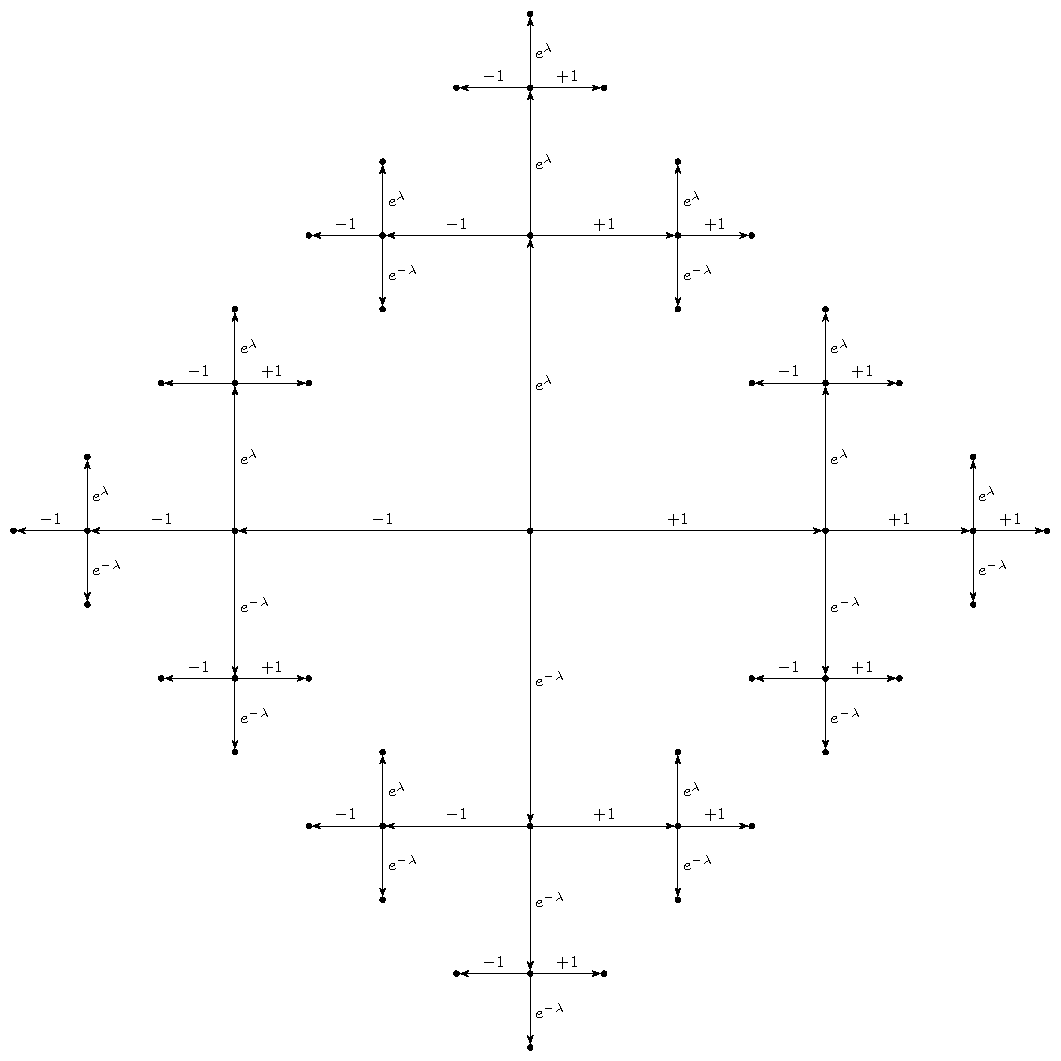
\includegraphics[width=3in]{images/cayley}
\caption{Cayley tree of syntactical structure}
\end{figure}

\begin{figure}[ht]
\centering
\begin{tikzpicture}

\filldraw [black] (0,0) circle (2pt) node[align=center, below] {0};
\filldraw [black] (4,1) circle (2pt) node[align=center, below] {$\alpha$};
\filldraw [black] (2,3) circle (2pt) node[align=center, below] {$\beta$};
\filldraw [black] (5,3) circle (2pt) node[align=center, below] {$\gamma$};
\filldraw [black] (-2,2) circle (2pt) node[align=center, below] {$\psi$};
\filldraw [black] (1,2) circle (2pt) node[align=center, below] {$\phi$};
\filldraw [gray] (3,-0.4) circle (0pt) node[align=center, below] {$x$};
\filldraw [gray] (3,1.8) circle (0pt) node[align=center, below] {$y$};
\filldraw [gray] (4.7,2) circle (0pt) node[align=center, below] {$z$};
\draw [gray] (0,0) to[out=300,in=240] (4,1);
\draw [gray] (4,1) to[out=120,in=300] (2,3);
\draw [gray] (4,1) to[out=60,in=240] (5,3);
\draw [gray] (0,0) to[out=120,in=300] (-2,2);
\draw [gray] (0,0) to[out=60,in=240] (1,2);
\filldraw [gray] (-1,0.8) circle (0pt) node[align=center, below] {$y$};
\filldraw [gray] (0.7,1) circle (0pt) node[align=center, below] {$z$};

\end{tikzpicture}
\caption{Factorization by greatest common divisor}
\end{figure}

The generating order is a partial order over $E$, we assume the later generated one is greater in generating.
By the generating order, we can define the concept of greatest common divisor: for any $\beta, \gamma \in A$,
the greatest common divisor $gcd(\beta, \gamma)$ is the greatest common ancestor in the generating tree.
So coprime of $\psi, \phi \in A$ means $gcd(\psi, \phi) = 0$

\begin{lemma}
\label{lemma:coprimes}
When $\alpha = gcd(\beta, \gamma)$, and $\beta = \alpha \circ \psi$, $\gamma = \alpha \circ \phi$ hold, then $\psi$ and $\phi$ are coprimes.
\end{lemma}

\subsection{Semantical structure}\label{sec:semantical}

Now we study the evaluation result, and the structure under the evaluation equality.
Giving an element of $E(\mu, \lambda)$ with a generating path $0 a_1 a_2 \cdots a_n$,
and the evaluation can be expressed by a function $\nu: E(\mu, \lambda) \to R$,
and we can proof by structure induction that all evaluation result keep the form

$$
\nu(0 a_1 a_2 \cdots a_n) = \sum_{i} k_i \mu e^{l_i \lambda} \in R
$$
where $k_i \in N, l_i \in N$, and obviously $\sum_{i} k_i \mu e^{l_i \lambda}$ is an evaluation of a polynomial over $\mathcal{F}$ at $e^{\lambda}$.
Comparing with path notion, we call this an expanded notion, or evaluated notion if we emphasising on evaluated value.

\begin{lemma}
\label{lemma:arithmeticalalgebra}
All arithmetical expressions $E(\mu, \lambda)$ is an algebra over numbers field $\mathcal{F}$, or $\mathcal{A} = (E, \mathcal{F}, \cdot)$.
\end{lemma}

\begin{proof}
By using the expanded notion, it is easy to verify the three axioms of an algebra is hold:
for any arithmetical expressions $x, y, z \in E$ and $a, b \in \mathcal{F}$, we have
\begin{itemize}
    \item right distributivity: $(x + y) \cdot z = x \cdot z + y \cdot z$
    \item left distributivity: $z \cdot (x + y) = z \cdot x + z \cdot y$
    \item compatibility with scalars: $(ax) \cdot (by) = (ab) (x \cdot y)$
\end{itemize}
\qedhere
\end{proof}

Since exponent appears in multiplication generators, we now study an equivalent formulation of Lindemann-Weierstrass theorem

\begin{theorem}
\label{theorem:LindemannWeierstrass}
If $\alpha_1, \cdots, \alpha_m$ are distinct algebraic numbers, then $e^{\alpha_1}, \cdots, e^{\alpha_m}$ are linearly independent over the algebraic numbers.
\end{theorem}

This theorem gives the transcendental nature of $e$.
Now we can verify path group $\mathcal{P}$ is non-abelian by calculating the result at point $0$ when the field $\mathcal{F}$ is algebraic.

\begin{corollary}
\label{corollary:nonabelian}
The path group $\mathcal{P} = (E, \circ)$ is non-abelian when the field $\mathcal{F}$ is algebraic
\end{corollary}

\begin{proof}
Because of Lindemann-Weierstrass theorem, $\mu$ have a covering structure and each layer of $\nu$ is a injectiion to the codomain.
Notice that $(0 + \mu) \cdot e^\lambda \neq 0 \cdot e^\lambda + \mu$, then we have $0 \oplus \otimes \neq 0 \otimes \oplus$
\qedhere
\end{proof}

\newpage

\section{Furthur reseach and problems}\label{sec:secondkind}

\subsection{Foundation questions}\label{sec:foundation}

\subsection{Eigenfunction problem}\label{sec:eigenfunction}

\subsection{Classification problem}\label{sec:donaghey}

\subsubsection{The second kind of arithmetic expression space}\label{sec:secondkind}

\subsubsection{The third kind of arithmetic expression space}\label{sec:thirdkind}

\subsection{Harmonic problem}\label{sec:tube}

\subsection{Tube structure}\label{sec:tube}

\subsection{Singular points and divergent series}\label{sec:tube}

\subsection{Function and Neo-caculus?}\label{sec:tube}

\subsection{Category of function theories?}\label{sec:tube}

\subsection{Geometrilization of computation and logic}\label{sec:tube}

\subsubsection{irrationality of $\sqrt{17}$}

\subsection{Questions related with complexity}\label{sec:tube}

\bibliography{aeg-paper.bib}

\appendix

\section{The grid}\label{sec:unitlength}

The grid in figure \ref{fig:grid} is power 2 based



\section{The direct solution of the flow equation}

\begin{equation}
    \frac{dx}{dt} = u(\mu \cos \theta + x \lambda \sin \theta)
\end{equation}

We can get the solution step by step:

\begin{equation}
    \frac{dx}{\mu \cos \theta + x \lambda \sin \theta} = u dt
\end{equation}

\begin{equation}
    \frac{1}{\lambda \sin \theta} \frac{d(\mu \cos \theta + x \lambda \sin \theta)}{\mu \cos \theta + x \lambda \sin \theta} = u dt
\end{equation}

\begin{equation}
    \frac{1}{\lambda \sin \theta} ln(\mu \cos \theta + x \lambda \sin \theta) = u t + C
\end{equation}

\begin{equation}
    \mu \cos \theta + x \lambda \sin \theta = e^{u \lambda t \sin \theta} e^{C \lambda \sin \theta}
\end{equation}

Considering the initial condition
\begin{equation}
    \mu \cos \theta + x_0 \lambda \sin \theta = e^{C \lambda \sin \theta}
\end{equation}

We have
\begin{equation}
    \mu \cos \theta + x \lambda \sin \theta = e^{u \lambda t \sin \theta} (\mu \cos \theta + x_0 \lambda \sin \theta)
\end{equation}

\begin{equation}
   x = \frac{\mu \cos \theta + x_0 \lambda \sin \theta}{\lambda \sin \theta} e^{\lambda t \sin \theta} - \frac{\mu}{\lambda}\cot \theta
\end{equation}

\begin{equation}
   x = (\frac{\mu}{\lambda} \cot \theta + x_0) e^{\lambda t \sin \theta} - \frac{\mu}{\lambda} \cot \theta
\end{equation}

\begin{equation}
   x =  x_0 e^{\lambda t \sin \theta} + \frac{\mu}{\lambda} (e^{\lambda t \sin \theta} - 1) \cot \theta
\end{equation}

In order to verify the conformance, we expand the formula

\begin{equation}
   x =  x_0 e^{\lambda t \sin \theta} + \frac{\mu}{\lambda} [1 + \lambda t \sin \theta + \frac{1}{2!} (\lambda t \sin \theta)^2  + \frac{1}{3!} (\lambda t \sin \theta)^3 + \cdots - 1] \cot \theta
\end{equation}

\begin{equation}
   x =  x_0 e^{\lambda t \sin \theta} + t \mu \cos \theta + \frac{\mu}{\lambda} \sin \theta \cos \theta (\frac{\lambda^2t^2}{2!} + \frac{\lambda^3t^3}{3!} \sin \theta + \frac{\lambda^4t^4}{4!} \sin^2 \theta + \cdots)
\end{equation}

\begin{equation}
   x =  x_0 e^{\lambda t \sin \theta} + t \mu \cos \theta + \frac{\mu}{2\lambda} \sin 2\theta (\frac{\lambda^2t^2}{2!} + \frac{\lambda^3t^3}{3!} \sin \theta + \frac{\lambda^4t^4}{4!} \sin^2 \theta + \cdots)
\end{equation}

\begin{equation}
   x =  x_0 e^{\lambda t \sin \theta} + \mu t \cos \theta + \frac{\mu}{2\lambda} \Psi(t) \sin 2\theta
\end{equation}

When $\theta = \frac{k \pi}{2}, k = 0, 1, 2, 3\cdots, t = 0, 1, 2, 3\cdots$, we have

\begin{equation}
    x = x_0 e^{\lambda t \sin \theta} + \mu t \cos \theta
\end{equation}

Especially, we have

\begin{equation}
    x = x_0 + \mu t, t = 0, 1, 2, 3\cdots, k = 0, 1, 2, 3\cdots, \theta = 2k\pi
\end{equation}

\begin{equation}
    x = x_0e^{\lambda t}, t = 0, 1, 2, 3\cdots, k = 0, 1, 2, 3\cdots, \theta = 2k\pi + \frac{\pi}{2}
\end{equation}

\begin{equation}
    x = x_0 - \mu t, t = 0, 1, 2, 3\cdots, k = 0, 1, 2, 3\cdots, \theta = 2k\pi + \pi
\end{equation}

\begin{equation}
    x = x_0 e^{- \lambda t}, t = 0, 1, 2, 3\cdots, k = 0, 1, 2, 3\cdots, \theta = 2k\pi + \frac{3 \pi}{2}
\end{equation}

which gives the conformance.

\section{Arithmetic expression, combinators and transformation over trees}\label{sec:expressions}

\subsection{LISP and combinators}\label{sec:donaghey}

\subsection{Applicative and concatenative}\label{sec:donaghey}

\subsection{Donaghey transformation}\label{sec:donaghey}

\newpage

\section{On order-4 apeirogonal tiling }\label{sec:secondkind}

\newpage


\end{document}
